\documentclass{article}
\usepackage{graphicx} % For including images
\usepackage{listings} % For including code
\usepackage{xcolor} % For syntax highligHing in code
\usepackage{float}
\title{Tugas Membuat Double Linked List}
\author{Rifqi Fadil Fahrial 1222646}
\date{\today}

\begin{document}

\maketitle

\section{Soal}
Buat program double link list untuk data mahasiswa dg fungsionalitas:  tambah
depan, tambah belakang,, hapus depan, hapus belakang, cari data, tampil data
dari head, tampil data dari tail.

\section{Hasil}
Program double linked list ini dibuat menggunakan bahasa c yang menampilkan
double link list untuk kemudahan dalam mengakses datanya
\begin{figure}[H]
\centering
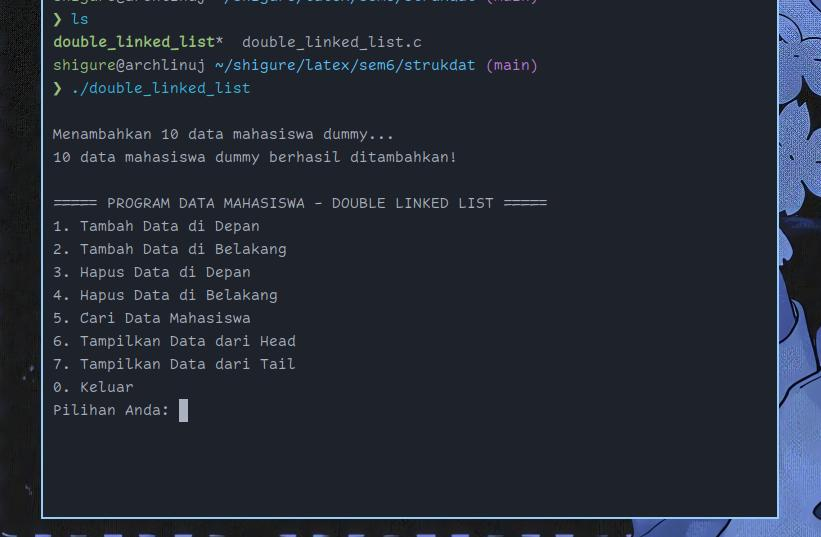
\includegraphics[width=0.5\textwidth]{images/gambar1.jpg}
\caption{Tampilan Utama}
\label{fig:sample-image}
\end{figure}

Aplikasi ini menginisialisasi 10 data dummy untuk mempermudah pengujian

\subsection{Menambahkan Data dari depan (HEAD)}

\begin{figure}[H]
\centering
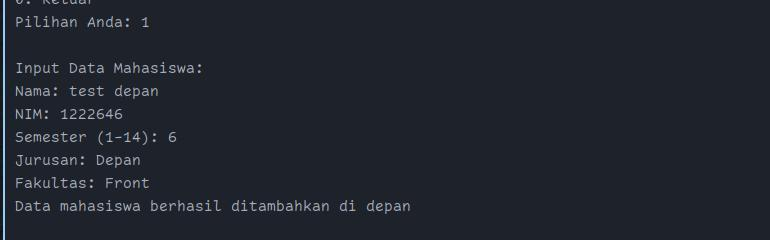
\includegraphics[width=0.9\textwidth]{images/gambar2.jpg}
\caption{Menambahkan Data dari depan (HEAD)}
\label{fig:sample-image}
\end{figure}

\subsection{Menambahkan Data dari belakang (TAIL)}

\begin{figure}[H]
\centering
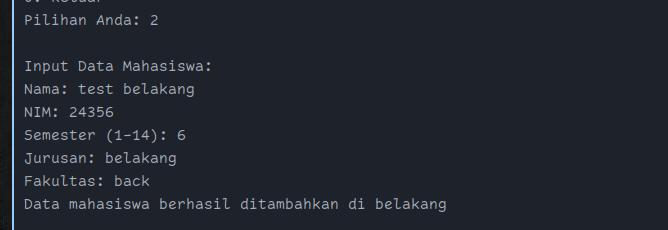
\includegraphics[width=0.9\textwidth]{images/gambar3.jpg}
\caption{Menambahkan Data dari belakang (TAIL)}
\label{fig:sample-image}
\end{figure}

\subsection{Mencari Mahasiswa dengan NIM}

\begin{figure}[H]
\centering
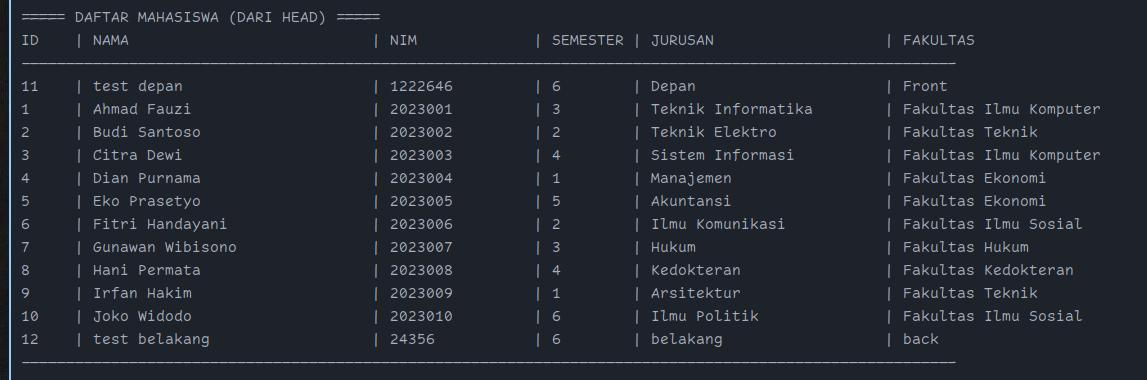
\includegraphics[width=0.9\textwidth]{images/gambar5.jpg}
\caption{Mencari Mahasiswa dengan NIM}
\label{fig:sample-image}
\end{figure}

\subsection{menampilkan mahasiswa dari head}

\begin{figure}[H]
\centering
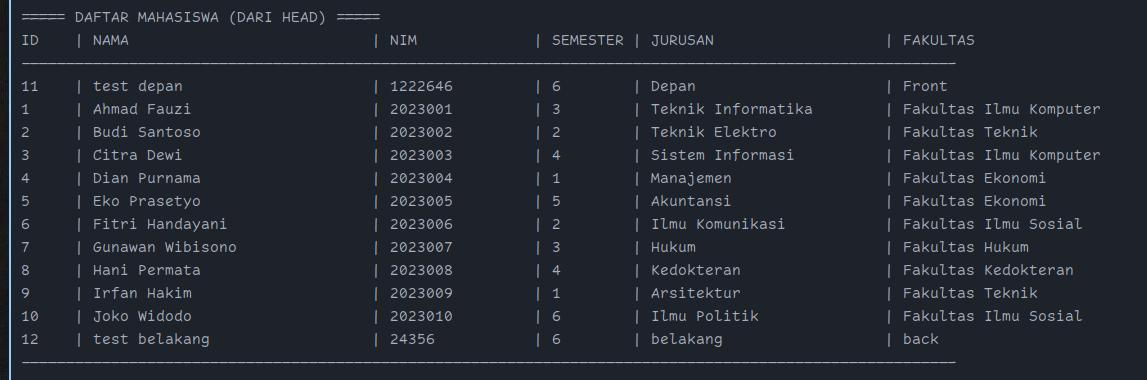
\includegraphics[width=0.9\textwidth]{images/gambar5.jpg}
\caption{menampilkan mahasiswa dari head}
\label{fig:sample-image}
\end{figure}

\subsection{menampilkan mahasiswa dari tail}

\begin{figure}[H]
\centering
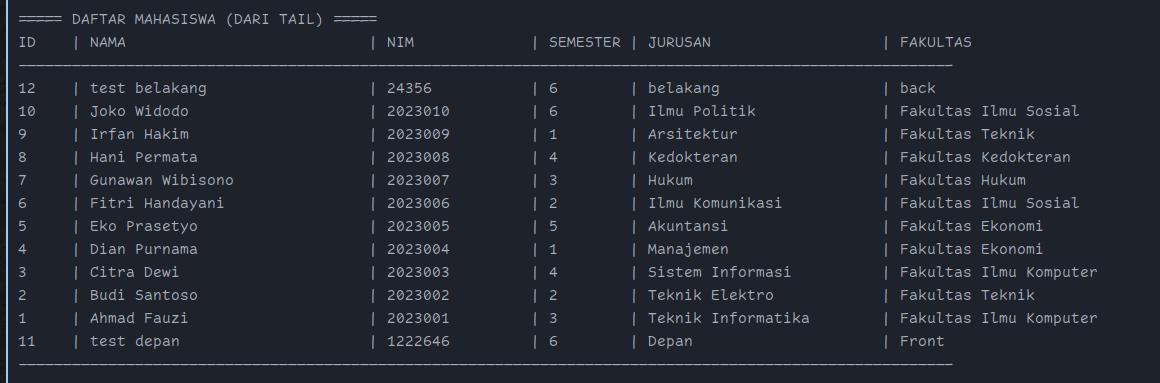
\includegraphics[width=0.9\textwidth]{images/gambar6.jpg}
\caption{menampilkan mahasiswa dari tail}
\label{fig:sample-image}
\end{figure}

\subsection{menghapus mahasiswa dari head}

\begin{figure}[H]
\centering
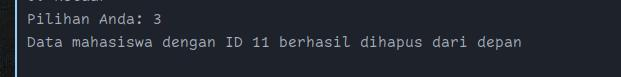
\includegraphics[width=0.9\textwidth]{images/gambar8.jpg}
\caption{menghapus mahasiswa dari head}
\label{fig:sample-image}
\end{figure}

\subsection{menghapus mahasiswa dari tail}

\begin{figure}[H]
\centering
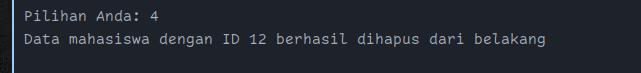
\includegraphics[width=0.9\textwidth]{images/gambar7.jpg}
\caption{menghapus mahasiswa dari tail}
\label{fig:sample-image}
\end{figure}

\subsection{menampilkan Hasil Akhir}

\begin{figure}[H]
\centering
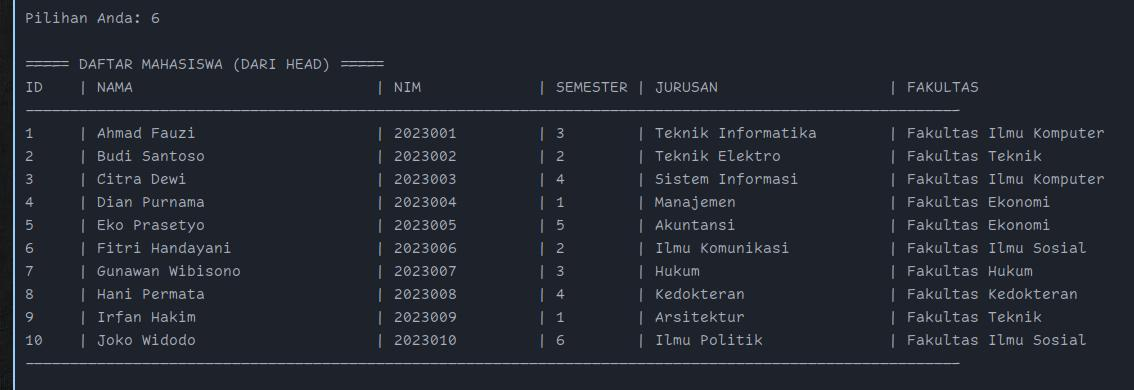
\includegraphics[width=0.9\textwidth]{images/gambar9.jpg}
\caption{menampilkan Hasil Akhir}
\label{fig:sample-image}
\end{figure}

\section{kode program}


\begin{lstlisting}[language=C, caption={Program Double Linked List},
  label={lst:sample-c-code}, basicstyle=\ttfamily\footnotesize,
  keywordstyle=\color{blue}, commentstyle=\color{green},
  stringstyle=\color{red}]
#include <stdio.h>
#include <stdlib.h>
#include <string.h>

// Struktur data untuk mahasiswa
typedef struct {
    int nomor_id;
    char nama[100];
    char nim[20];
    int semester;
    char jurusan[100];
    char fakultas[100];
} Mahasiswa;

// Struktur node untuk double linked list
typedef struct Node {
    Mahasiswa data;
    struct Node *prev;
    struct Node *next;
} Node;

// Fungsi untuk membuat node baru
Node* buatNode(Mahasiswa data) {
    Node* newNode = (Node*)malloc(sizeof(Node));
    if (newNode == NULL) {
        printf("Alokasi memori gagal\n");
        exit(1);
    }
    
    newNode->data = data;
    newNode->prev = NULL;
    newNode->next = NULL;
    
    return newNode;
}

// Fungsi untuk menambah node di depan
void tambahDepan(Node** head, Node** tail, Mahasiswa data) {
    Node* newNode = buatNode(data);
    
    if (*head == NULL) {
        // Jika list kosong
        *head = newNode;
        *tail = newNode;
        return;
    }
    
    newNode->next = *head;
    (*head)->prev = newNode;
    *head = newNode;
}

// Fungsi untuk menambah node di belakang
void tambahBelakang(Node** head, Node** tail, Mahasiswa data) {
    Node* newNode = buatNode(data);
    
    if (*head == NULL) {
        // Jika list kosong
        *head = newNode;
        *tail = newNode;
        return;
    }
    
    (*tail)->next = newNode;
    newNode->prev = *tail;
    *tail = newNode;
}

// Fungsi untuk menghapus node di depan
int hapusDepan(Node** head, Node** tail) {
    if (*head == NULL) {
        printf("List kosong, tidak ada yang bisa dihapus\n");
        return 0;
    }
    
    Node* temp = *head;
    
    if (*head == *tail) {
        // Jika hanya ada satu node
        *head = NULL;
        *tail = NULL;
    } else {
        *head = (*head)->next;
        (*head)->prev = NULL;
    }
    
    printf("Data mahasiswa dengan ID %d berhasil dihapus dari depan\n", temp->data.nomor_id);
    free(temp);
    return 1;
}

// Fungsi untuk menghapus node di belakang
int hapusBelakang(Node** head, Node** tail) {
    if (*head == NULL) {
        printf("List kosong, tidak ada yang bisa dihapus\n");
        return 0;
    }
    
    Node* temp = *tail;
    
    if (*head == *tail) {
        // Jika hanya ada satu node
        *head = NULL;
        *tail = NULL;
    } else {
        *tail = (*tail)->prev;
        (*tail)->next = NULL;
    }
    
    printf("Data mahasiswa dengan ID %d berhasil dihapus dari belakang\n", temp->data.nomor_id);
    free(temp);
    return 1;
}

// Fungsi untuk mencari data berdasarkan NIM
Node* cariData(Node* head, char* nim) {
    Node* current = head;
    
    while (current != NULL) {
        if (strcmp(current->data.nim, nim) == 0) {
            return current;
        }
        current = current->next;
    }
    
    return NULL; // Data tidak ditemukan
}

// Fungsi untuk menampilkan data dari head
void tampilDariHead(Node* head) {
    if (head == NULL) {
        printf("List kosong\n");
        return;
    }
    
    printf("\n===== DAFTAR MAHASISWA (DARI HEAD) =====\n");
    printf("%-5s | %-30s | %-15s | %-8s | %-25s | %-25s\n", "ID", "NAMA", "NIM", "SEMESTER", "JURUSAN", "FAKULTAS");
    printf("--------------------------------------------------------------------------------------------------------\n");
    
    Node* current = head;
    while (current != NULL) {
        printf("%-5d | %-30s | %-15s | %-8d | %-25s | %-25s\n",
               current->data.nomor_id,
               current->data.nama,
               current->data.nim,
               current->data.semester,
               current->data.jurusan,
               current->data.fakultas);
        current = current->next;
    }
    printf("--------------------------------------------------------------------------------------------------------\n");
}

// Fungsi untuk menampilkan data dari tail
void tampilDariTail(Node* tail) {
    if (tail == NULL) {
        printf("List kosong\n");
        return;
    }
    
    printf("\n===== DAFTAR MAHASISWA (DARI TAIL) =====\n");
    printf("%-5s | %-30s | %-15s | %-8s | %-25s | %-25s\n", "ID", "NAMA", "NIM", "SEMESTER", "JURUSAN", "FAKULTAS");
    printf("--------------------------------------------------------------------------------------------------------\n");
    
    Node* current = tail;
    while (current != NULL) {
        printf("%-5d | %-30s | %-15s | %-8d | %-25s | %-25s\n",
               current->data.nomor_id,
               current->data.nama,
               current->data.nim,
               current->data.semester,
               current->data.jurusan,
               current->data.fakultas);
        current = current->prev;
    }
    printf("--------------------------------------------------------------------------------------------------------\n");
}

// Fungsi untuk menambahkan 10 data mahasiswa dummy untuk pengujian
void tambahDummyData(Node** head, Node** tail, int* idCounter) {
    Mahasiswa dummy[10] = {
        {0, "Ahmad Fauzi", "2023001", 3, "Teknik Informatika", "Fakultas Ilmu Komputer"},
        {0, "Budi Santoso", "2023002", 2, "Teknik Elektro", "Fakultas Teknik"},
        {0, "Citra Dewi", "2023003", 4, "Sistem Informasi", "Fakultas Ilmu Komputer"},
        {0, "Dian Purnama", "2023004", 1, "Manajemen", "Fakultas Ekonomi"},
        {0, "Eko Prasetyo", "2023005", 5, "Akuntansi", "Fakultas Ekonomi"},
        {0, "Fitri Handayani", "2023006", 2, "Ilmu Komunikasi", "Fakultas Ilmu Sosial"},
        {0, "Gunawan Wibisono", "2023007", 3, "Hukum", "Fakultas Hukum"},
        {0, "Hani Permata", "2023008", 4, "Kedokteran", "Fakultas Kedokteran"},
        {0, "Irfan Hakim", "2023009", 1, "Arsitektur", "Fakultas Teknik"},
        {0, "Joko Widodo", "2023010", 6, "Ilmu Politik", "Fakultas Ilmu Sosial"}
    };
    
    printf("\nMenambahkan 10 data mahasiswa dummy...\n");
    
    for (int i = 0; i < 10; i++) {
        dummy[i].nomor_id = (*idCounter)++;
        tambahBelakang(head, tail, dummy[i]);
    }
    
    printf("10 data mahasiswa dummy berhasil ditambahkan!\n");
}

// Fungsi untuk membersihkan memori yang dialokasikan untuk list
void hapusList(Node** head, Node** tail) {
    Node* current = *head;
    Node* next;
    
    while (current != NULL) {
        next = current->next;
        free(current);
        current = next;
    }
    
    *head = NULL;
    *tail = NULL;
}

int main() {
    Node* head = NULL;
    Node* tail = NULL;
    
    int pilihan;
    int idCounter = 1;
    Mahasiswa mhs;
    char nimCari[20];

    //inisialisasi data dummy
    tambahDummyData(&head, &tail, &idCounter);
    
    do {
        printf("\n===== PROGRAM DATA MAHASISWA - DOUBLE LINKED LIST =====\n");
        printf("1. Tambah Data di Depan\n");
        printf("2. Tambah Data di Belakang\n");
        printf("3. Hapus Data di Depan\n");
        printf("4. Hapus Data di Belakang\n");
        printf("5. Cari Data Mahasiswa\n");
        printf("6. Tampilkan Data dari Head\n");
        printf("7. Tampilkan Data dari Tail\n");
        printf("0. Keluar\n");
        printf("Pilihan Anda: ");
        scanf("%d", &pilihan);
        getchar(); // Membersihkan buffer
        
        switch(pilihan) {
            case 1: // Tambah Depan
                mhs.nomor_id = idCounter++;
                
                printf("\nInput Data Mahasiswa:\n");
                printf("Nama: ");
                fgets(mhs.nama, sizeof(mhs.nama), stdin);
                mhs.nama[strcspn(mhs.nama, "\n")] = '\0'; // Hapus newline
                
                printf("NIM: ");
                fgets(mhs.nim, sizeof(mhs.nim), stdin);
                mhs.nim[strcspn(mhs.nim, "\n")] = '\0'; // Hapus newline
                
                printf("Semester (1-14): ");
                scanf("%d", &mhs.semester);
                getchar(); // Membersihkan buffer
                
                printf("Jurusan: ");
                fgets(mhs.jurusan, sizeof(mhs.jurusan), stdin);
                mhs.jurusan[strcspn(mhs.jurusan, "\n")] = '\0'; // Hapus newline
                
                printf("Fakultas: ");
                fgets(mhs.fakultas, sizeof(mhs.fakultas), stdin);
                mhs.fakultas[strcspn(mhs.fakultas, "\n")] = '\0'; // Hapus newline
                
                tambahDepan(&head, &tail, mhs);
                printf("Data mahasiswa berhasil ditambahkan di depan\n");
                break;
                
            case 2: // Tambah Belakang
                mhs.nomor_id = idCounter++;
                
                printf("\nInput Data Mahasiswa:\n");
                printf("Nama: ");
                fgets(mhs.nama, sizeof(mhs.nama), stdin);
                mhs.nama[strcspn(mhs.nama, "\n")] = '\0'; // Hapus newline
                
                printf("NIM: ");
                fgets(mhs.nim, sizeof(mhs.nim), stdin);
                mhs.nim[strcspn(mhs.nim, "\n")] = '\0'; // Hapus newline
                
                printf("Semester (1-14): ");
                scanf("%d", &mhs.semester);
                getchar(); // Membersihkan buffer
                
                printf("Jurusan: ");
                fgets(mhs.jurusan, sizeof(mhs.jurusan), stdin);
                mhs.jurusan[strcspn(mhs.jurusan, "\n")] = '\0'; // Hapus newline
                
                printf("Fakultas: ");
                fgets(mhs.fakultas, sizeof(mhs.fakultas), stdin);
                mhs.fakultas[strcspn(mhs.fakultas, "\n")] = '\0'; // Hapus newline
                
                tambahBelakang(&head, &tail, mhs);
                printf("Data mahasiswa berhasil ditambahkan di belakang\n");
                break;
                
            case 3: // Hapus Depan
                hapusDepan(&head, &tail);
                break;
                
            case 4: // Hapus Belakang
                hapusBelakang(&head, &tail);
                break;
                
            case 5: // Cari Data
                printf("Masukkan NIM mahasiswa yang dicari: ");
                fgets(nimCari, sizeof(nimCari), stdin);
                nimCari[strcspn(nimCari, "\n")] = '\0'; // Hapus newline
                
                Node* hasil = cariData(head, nimCari);
                
                if (hasil != NULL) {
                    printf("\n===== DATA MAHASISWA DITEMUKAN =====\n");
                    printf("ID      : %d\n", hasil->data.nomor_id);
                    printf("Nama    : %s\n", hasil->data.nama);
                    printf("NIM     : %s\n", hasil->data.nim);
                    printf("Semester: %d\n", hasil->data.semester);
                    printf("Jurusan : %s\n", hasil->data.jurusan);
                    printf("Fakultas: %s\n", hasil->data.fakultas);
                } else {
                    printf("Data mahasiswa dengan NIM %s tidak ditemukan\n", nimCari);
                }
                break;
                
            case 6: // Tampilkan dari Head
                tampilDariHead(head);
                break;
                
            case 7: // Tampilkan dari Tail
                tampilDariTail(tail);
                break;
            case 0: // Keluar
                printf("Terima kasih telah menggunakan program ini\n");
                break;
                
            default:
                printf("Pilihan tidak valid. Silakan coba lagi.\n");
        }
    } while (pilihan != 0);
    
    // Membersihkan memori sebelum keluar
    hapusList(&head, &tail);
    
    return 0;
}

\end{lstlisting}

\end{document}
